%-*- tex-command: "pdflatex" -*-
\documentclass{llncs}
\usepackage{graphicx}
\usepackage{float}
\usepackage{enumerate}
\usepackage{amssymb,amsmath}
\usepackage{enumitem}
\usepackage{verbatim}

\newcommand{\norm}[1]{\left\| #1 \right\|}

\begin{document}

\title{On the State Complexity of Ultrametric Finite Automata}


\author{
Kaspars Balodis,
Anda Beri\c na,
Krist\= \i ne C\= \i pola,
Maksims Dimitrijevs,
J\= anis Iraids,
K\= arlis J\= eri\c n\v s,
Vladimirs Kacs,
J\= anis Kal\= ejs,
Rihards Kri\v slauks,
K\= arlis Luksti\c n\v s,
Reinholds Raumanis,
Nat\= alija Somova,
Irina \v S\v cegu\c lnaja,
Anna Vanaga,
R\= usi\c n\v s Freivalds}
\institute{Institute of Mathematics and Computer Science,
 University of Latvia,\\ Rai\c na bulv\= aris 29, Riga, LV-1459, Latvia
}



\maketitle

\begin{abstract}  
We investigate ultrametric finite automata using $p$-adic numbers to describe random branching of the process of computation. These automata have properties similar to the properties of probabilistic automata but the descriptional power of probabilistic automata and ultrametric automata can differ very much.
\end{abstract} 



\section{Introduction} 

Pascal and Fermat believed that every event of indeterminism can be described by a real number between 0 and 1 called 
{\em probability}. Quantum physics introduced a description in terms of complex numbers called {\em amplitude of 
probabilities} and later in terms of probabilistic combinations of amplitudes most conveniently described by {\em density
matrices}.

String theory \cite{VVZ95}, chemistry \cite{K06} and molecular biology \cite{DD09,Kh97} have introduced $p$-adic numbers to describe
measures of indeterminism. 

There were no difficulties to implement probabilistic automata and algorithms practically. Quantum computation \cite{H01}  has made a considerable
theoretical progress but practical implementation has met considerable difficulties. However, prototypes of quantum computers exist, some
quantum algorithms are implemented on these prototypes, quantum cryptography is already practically used. Some people are skeptical concerning
practicality of the initial spectacular promises of quantum computation but nobody can deny the existence of quantum computation.

We consider a new type of indeterministic algorithms called {\em ultrametric} algorithms. They are very similar to probabilistic algorithms but while probabilistic algorithms use real numbers $r$ with $0 \leq r \leq 1$ as parameters, ultrametric algorithms use {\em $p$-adic} numbers.
Slightly simplifying the description of the definitions one can say that ultrametric algorithms are the same probabilistic algorithms, only the interpretation of the probabilities is different. 

Our choice of $p$-adic numbers instead of real numbers is not quite arbitrary. In 1916 Alexander Ostrowski 
proved that any non-trivial absolute value on the rational numbers $Q$ is equivalent to either the usual real absolute value or a $p$-adic absolute value.
This result shows that using $p$-adic numbers is not merely one of many possibilities to generalize the definition of deterministic algorithms but rather the only remaining possibility not yet explored.

Moreover, Helmut Hasse's local-global principle
 states that certain types of equations have a rational solution if and only if they have a solution in the real numbers and in the $p$-adic numbers for each prime $p$.

For every prime number $p$ there exists a different notion of absolute value in the set of rational numbers. These absolute values are traditionally  called {\em ultrametric}. 
Absolute values are needed to consider {\em distances} among objects. We are used to rational and irrational numbers as measures for distances, and there is a psychological difficulty to imagine that something else can be used instead of irrational numbers.
However, there is an important feature that distinguishes $p$-adic numbers from real numbers. Real numbers (both rational and irrational) are linearly ordered.
$p$-adic numbers cannot be linearly ordered. This is why {\em valuations} of $p$-adic numbers are considered. 

The situation is similar in Quantum Computation. Quantum amplitudes are complex numbers which also cannot be linearly ordered. The counterpart of valuation for quantum algorithms is {\em measurement} translating a complex number $a + bi$ into a real number $a^2 + b^2$. Valuations of $p$-adic numbers are rational numbers.

\section{$p$-adic numbers}

In describing the notion of {\em p-adic numbers} we follow the introductory text by David A. Madore \cite{M00}.

Let $p$ be an arbitrary prime number. A $p$-adic digit is a natural number between $0$ and $p-1$ (inclusive). A $p$-adic integer is by definition a sequence $(a_i)_{i \in \mathbb{N}}$ of $p$-adic digits. We write this conventionally as
$$
\cdots a_i \cdots  a_2 a_1 a_0
$$
(that is, the $a_i$ are written from right to left).

If $n$ is a natural number, and
$$
n = \overline{a_{k-1} a_{k-2} \cdots  a_1 a_0}
$$
is its $p$-adic representation (in other words $n = \sum ^{k-1}_{i=0}  a_ip^i$ with each $a_i$ a $p$-adic digit) then we identify $n$ with the $p$-adic integer $(a_i)$ with $a_i = 0$ if $i \geq k$. This means that natural numbers coincide with $p$-adic integers with a finite number of nonzero digits. Also note that $0$ is the $p$-adic integer all of whose digits are $0$, and that $1$ is the $p$-adic integer all of whose digits are $0$ except the right-most one which is $1$.
If $\alpha  = (a_i)$ and $\beta = (b_i)$ are two $p$-adic integers, we will now define their sum. To this purpose, we define by induction a sequence $(c_i)$ of $p$-adic digits and a sequence $(\epsilon _i)$ of elements of $\{0, 1\}$ (the "carries") as follows:


\begin{itemize}
  \item  $\epsilon _0$ is $0.$
  \item  $c_i$ is $a_i + b_i + \epsilon _i$ or $a_i + b_i + \epsilon _i - p$ according as which of these two is a $p$-adic digit. In the former case, $\epsilon _{i+1} = 0$ and in the latter, $\epsilon _{i+1} = 1.$
\end{itemize}


Under those circumstances, we let $\alpha + \beta = (c_i)$ and we call $\alpha + \beta $ the sum of $\alpha $ and $\beta $. Note that the rules described above are exactly the rules used for adding natural numbers in base $p$. In particular, if $\alpha $ and $\beta $ turn out to be natural numbers, then their sum as a $p$-adic integer is no different from their sum as a natural number. Addition is therefore associative and commutative.
Similarly, subtraction and multiplication of $p$-adic integers is done exactly the same as with natural numbers in base $p$.

Division of $p$-adics, however, cannot always be performed. For example, $\frac{1}{p}$ has no meaning as a $p$-adic integer - that is, the equation $p\alpha  = 1$  has no solution - since multiplying a $p$-adic integer by $p$ always gives a $p$-adic integer ending in $0$. There is nothing really surprising here: $\frac{1}{p}$ cannot be performed in the integers either.
However, what is mildly surprising is that division by $p$ is essentially the only division which cannot be performed in the $p$-adic integers.  This is one of the reasons why the notion of
$p$-adic integers is generalized and {\em $p$-adic numbers} are introduced. They are formal sequences of $p$-adic digits such that the sequence is infinite in the left-hand direction but finite in the right-hand direction. The notion of {\em $p$-adic dot} is introduced. The set of all $p$-adic numbers is denoted by 
$Q_p$.

For example, with $p = 7$ we show that the number $\alpha  = \cdots  333334$  is the number $\frac{1}{2}$ by adding it to it itself:
$$
\begin{tabular}{rrrrrrrrr|}
$\cdots$ &3 &3 &3 &3 &3 &4\\
$\cdots$ &3 &3 &3 &3 &3 &4\\
\hline
\hline
$\cdots$ &0 &0 &0 &0 &0 &1\\
\hline
\end{tabular}
$$
Thus, in the 7-adic numbers, $\frac{1}{2}$ is an integer. And so are $\frac{1}{3}$ $(\cdots 44445)$, $\frac{1}{4}$ $(\cdots 1515152)$, $\frac{1}{5}$ $(\cdots 541254125413)$, $\frac{1}{6}$ $(\cdots 55556)$, $\frac{1}{8}$ $(\cdots 0606061)$, and so on.
But $\frac{1}{7}$, $\frac{1}{14}$ and so on, are not 7-adic integers. They are expressed as follows.
$$
\begin{tabular}{rrrrrrrr|}
$\cdots$ &0&0&0&0&.&1\\
\end{tabular}
$$
$$
\begin{tabular}{rrrrrrrrr|}
$\cdots$ &0&0&0&0&.&0&1\\
\end{tabular}
$$
It is important to notice that $p$-adic numbers that are not $p$-adic integers and irrational real numbers are kind of incompatible. It is known that no $p$-adic number corresponds to $\sqrt{2}, \pi , e$ and there is a continuum of $p$-adic numbers not corresponding to any real number. Moreover, if $p_1 \neq p_2$ then $p_1$-adic and $p_2$-adic numbers are also incompatible.

However, $p$-adic numbers is not merely a generalization of rational numbers. They are very special because of the notion of {\em absolute value} of numbers.

If $X$ is a nonempty set, a distance, or {metric}, on $X$ is a function $d$ from pairs of elements $(x,y)$ of $X$ to the nonnegative real numbers such that
\begin{enumerate}[itemsep=9pt]
\item $d(x,y) = 0$ if and only if $x = y$,
\item $d(x,y) = d(y,x)$,
\item $d(x,y) \leq d(x,z) + d(z,y)$ for all $z \in X$.
\end{enumerate}

A set $X$ together with a metric $d$ is called a {\em metric space}. The same set $X$ can be equipped with several different metrics.


The {\em norm} of an element $x \in X$ denoted $\norm{x}$ is its distance from $0$:
\begin{enumerate}[itemsep=9pt]
\item $\norm{x} = 0$ if and only if $x = 0$,
\item $\norm{x \cdot y} = \norm{x} \cdot \norm{y} $,
\item $\norm{x+y} \leq \norm{x}+\norm{y} $.
\end{enumerate}

A norm  is called {\em ultrametric}  if the third requirement can be replaced by the stronger statement:
$\norm{x+y} \leq \max \{\norm{x}, \norm{y} \}$.
Otherwise, the norm is called {\em Archimedean}.

\begin{definition}
Let $p$ be any prime number. For any nonzero integer $a$, let the $p$-adic ordinal (or valuation) of $a$, denoted $ord_p a$, be the highest power of $p$ which divides $a$, i.e., the greatest $m$ such that $a \equiv 0 \pmod{p^{m}}$. For any rational number $x = a/b$, denote $ord_p x$ to be $ord_p a - ord_p b$. Additionally, $ord_p x = \infty $ if and only if $x = 0$.
\end{definition}

For example, the 7-adic valuation of 7 is 1. That of 14 is also 1, as are those of 21, 28, 35, 42 or 56. The 7-adic valuation of 49, on the other hand, is 2, as is that of 98. And the 7-adic valuation of 343 is 3. The 2-adic valuation of an integer is 0 iff it is odd, it is at least 1 iff it is even, at least 2 iff the integer is multiple by 4, and so on. The 7-adic valuation of $\frac{1}{7}$ is -1, and so are those of $\frac{3}{7}$, $\frac{1}{14}$, $\frac{5}{56}$. The 7-adic valuation of $\frac{1}{2}$ or $\frac{8}{3}$ is 0. The 7-adic valuation of $\frac{7}{3}$ or $\frac{14}{5}$ is 1. The 7-adic valuation of $\frac{48}{49}$ is -2.

\begin{definition}
Let $p$ be any prime number. For arbitrary rational number $x$, its {\em $p$-norm} is:
\[|x|_p = \begin{cases}
  \frac{1}{p^{ord_p x}}, &\text{ if } x \neq 0;\\
  0, &\text{ if } x = 0.
\end{cases}\]
\end{definition}

For example, $|p|_p = \frac{1}{p} , |1|_p = 1, |2p|_p = \frac{1}{p}$ ( if $p$ is odd), and $|\frac{1}{p^2}| = p^2$.

It is easy to see that the valuation of a $p$-adic number $(a_i)$ is the greatest $i_0$ such that $a_i = 0$ for all $i < i_0$. Hence a $p$-adic integer is exactly a $p$-adic number with non negative valuation. And a small $p$-adic integer (one which ends in 0) is one whose valuation is (strictly) positive. It is not hard to check that this definition coincides with the aforementioned one for integers, hence for rationals. As for rationals, we define the $p$-adic absolute value and distance by $|\alpha |_p = p^{- ord_p \alpha }$. Note that the $p$-adic absolute value of a $p$-adic number is a real number (it is also a $p$-adic, and in fact a rational, but ought not to be considered as such).

Every rational number is a $p$-adic number for some prime number $p$. The nature of irrational numbers is more complicated. For instance, $\sqrt{2}$ just does not exist as a $p$-adic number. On the other hand, there is a of continuum of $p$-adic numbers that are not real numbers. Also, for different primes $p_1$, $p_2$ there is a continuum of $p_1$-adic numbers not being $p_2$-adic numbers, and vice versa.

\section{$p$-adic automata}


The notion of $p$-adic numbers is widely used in mathematics but not so much in Computer Science. The aim of our next sections is to show that the notion of ultrametric automata is natural. 

In mathematics, a stochastic matrix  is a matrix used to describe the transitions of a Markov chain. A {\em right stochastic matrix}  is a square matrix each of whose rows consists of nonnegative real numbers, with each row summing to 1. A {\em stochastic vector} is a vector whose elements consist of nonnegative real numbers which sum to 1. The {\em finite probabilistic automaton} is defined as an extension of a non-deterministic finite automaton $(Q,\Sigma,\delta,q_0,F)$,  with the initial state $q_0$ replaced by a stochastic vector giving the probability of the automaton being in a given initial state, and with stochastic matrices corresponding to each symbol in the input alphabet describing the state transition probabilities. It is important to note that if $A$ is the stochastic matrix corresponding to the input symbol $a$ and $B$ is the stochastic matrix corresponding to the input symbol $b$, then the product $AB$ describes the state transition probabilities when the automaton reads the input word $ab$. Additionally, the probabilistic automaton has a threshold $\lambda $ being a real number between 0 and 1. If the probabilistic automaton has only one {\em final state} then the input word $x$ is said to be accepted if after reading $x$ the probability of the final state has a probability exceeding $\lambda $. If there are several final states, the word $x$ is said to be accepted if the total of probabilities of the final states exceeds $\lambda $.

Ultrametric automata (introduced by Freivalds in \cite{F12}) are defined exactly in the same way as probabilistic automata, only the parameters called {\em probabilities of transition}  from one state to another one are real numbers between 0 and 1 in probabilistic automata, and they are $p$-adic numbers called {\em amplitudes} in the ultrametric automata. Formulas to calculate the amplitudes after one, two, three, $\cdots $ steps of computation are exactly the same as the formulas to calculate the probabilities in the probabilistic automata. At the beginning of the work, the states of the automaton get {\em initial amplitudes} being $p$-adic numbers. When reading the current symbol of the input word, the automaton changes the amplitudes of all the states according to the transition matrix corresponding to this input symbol. 
After reading the input word, the {\em measurement} is performed, and the  amplitudes of all the states are transformed into the $p$-valuations of these amplitudes. The valuations are real numbers and it is possible to compare whether or not the valuation exceed the threshold $\lambda $.

Paavo Turakainen considered various generalizations of finite probabilistic automata in 1969 and proved that there is no need to demand in cases of probabilistic branchings that total of probabilities for all possible continuations equal 1 \cite{T69}. He defined generalized probabilistic finite automata where the "probabilities" can be arbitrary real numbers, and that languages recognizable by these generalized probabilistic finite automata are the same as for ordinary probabilistic finite automata. Hence we also allow usage of all possible $p$-adic numbers in $p$-ultrametric machines.

However, it is needed to note that if there is only one final state then the possible probabilities of acceptance are discrete values $0$, $p^1$, $p^{-1}$, $p^2$, $p^{-2}$, $p^3$, $p^{-3}$, $\cdots $. Hence there is no natural counterpart of {\em isolated cut-point} or {\em bounded error} for ultrametric machines. On the other hand, a counterpart of Turakainen's theorem for isolated cut-point still does not exist. We also did not succeed to prove such a theorem for ultrametric automata. Most probably, there are certain objective difficulties.

\begin{definition}
A finite $p$-ultrametric automaton is a sextuple $\langle S, \Sigma, s_0, \delta, F, \Lambda \rangle$, where
\begin{itemize}
  \item $S$ is a finite set -- the set of states,
  \item $\Sigma$ is a finite set, ($\$ \notin \Sigma$) -- the input alphabet,
  \item $s_0:S \rightarrow Q_p$ is the initial amplitude distribution,
  \item $\delta: \left( \Sigma \cup \left\{ \$ \right\} \right) \times S \times S \rightarrow Q_p$ is the transition function,
  \item $F \subseteq S$ is the set of final states,
  \item $\Lambda = \left( \lambda, \diamond \right)$ is the acceptance condition where $\lambda \in \mathbb{R}$ is the acceptance threshold and $\diamond \in \left\{ \leq, \geq \right\}$.
\end{itemize}
The automaton works as follows.
At every timestep each of its states has an associated $p$-adic number called its amplitude.
The automaton starts with the initial amplitude distribution $s_0$.
Then it proceeds by processing input word's $w = w_1 \ldots w_n$ symbols one by one.
The amplitude distribution after processing the $i$-th symbol is denoted as $s_i$, with
$s_i(y) = \sum_{x \in S}{s_{i-1}(x) \cdot \delta \left( w_i, x, y \right) }$ for every $y \in S$.
After the $n$-th symbol, in the same way the end marker $\$$ is processed obtaining the final amplitude distribution $s_{n+1}$.
If the sum of the $p$-norms of final amplitudes over final states is at least (or at most) the threshold, i.e., if $\sum_{x \in F}{\left| s_{n+1}(x) \right|_p} \diamond \lambda$, then the word $w$ is said to be accepted, otherwise -- rejected.
\end{definition}

\begin{definition}
We say that a finite $p$-ultrametric automaton {\bf recognizes} language $L \subseteq \Sigma^{*}$ if any word $w \in  \Sigma^{*}$ is accepted if and only if $w \in L$.
\end{definition}

It is sometimes useful to describe a state of the automaton as an $|S|$-dimensi\-onal row vector $s$ and the transition function as a set of $|\Sigma|$ matrices $\{A_\sigma\}$ with $(A_\sigma)_{xy}=\delta(\sigma, x, y)$. Then the state after reading the word $\sigma_1\sigma_2\ldots \sigma_n$ is simply $s_0\cdot M_{\sigma_1} \cdot M_{\sigma_2} \cdot \ldots \cdot M_{\sigma_n}$.

\begin{definition}
Finite $p$-ultrametric automaton is called {\bf integral} if all the $p$-adic numbers in its initial distribution $s_0$ and transition function $\delta$ are $p$-adic integers.
\end{definition}

\begin{comment}
\begin{definition}
A square matrix with elements being $p$-adic numbers is called {\bf balanced} if for arbitrary row of the matrix the product of $p$-norms of the elements equals 1.
\end{definition}

\begin{definition}
A finite $p$-ultrametric automaton is called {\bf balanced} if all the matrices in its definition are balanced.
\end{definition}

\begin{theorem}
If a language $M$ can be recognized by a finite ultrametric automaton then $M$ can be recognized also by a balanced finite ultrametric automaton.
\end{theorem}

\begin{proof}
For every state of the automaton we add its duplicate. If the given state has an amplitude $\gamma $ then its duplicate has the amplitude $\frac{1}{\gamma }$.
\end{proof}
\end{comment}

\begin{definition}
A state of a $p$-ultrametric automaton is called {\bf regulated} if there exist constants $\rho$, $c$ such that for every input word the $p$-norm of amplitude $\gamma$ of this state is bounded by $0 < \rho -c < |\gamma |_p < \rho +c$.

A finite $p$-ultrametric automaton is called {\bf regulated} if all of its states are regulated (it is not required for the constants $\rho$ and $c$ to be the same for all states).
\end{definition}

We show a gap between state complexity of deterministic and ultrametric automata.

Let $w = \left( w_1, \ldots, w_m \right) \in \left\{ 0, 1, \ldots, k-1 \right\} ^ m$.
We consider two operations:
\begin{enumerate}[itemsep=9pt,label=\alph*)]
  \item a cyclic shift: $f_a \left( w_1, w_2, \ldots, w_{m} \right) = \left( w_{m}, w_1, w_2, \ldots, w_{m-1} \right)$.
  \item increasing the first element: $f_b \left( w_1, w_2, \ldots, w_{m} \right) = ( \left( w_1 + 1 \right) \bmod k, w_2,\ldots, \allowbreak w_{m} )$.
\end{enumerate}


Let $x \in \left\{ a, b \right\} ^n$. We define $f_{x_1 x_2 \ldots x_n} \left( w \right) = f_{x_n} \left( \cdots f_{x_2} \left( f_{x_1} \left( w \right) \right) \cdots \right)$.

We consider the following language
$$
L_{k,m} = \left\{ x \in \left\{ a, b \right\}^* \left| f_x(0^m) = 0^m \right.  \right\}
$$


\begin{theorem}
Every deterministic finite automaton recognizing $L_{k,m}$ needs at least $k^m$ states.
\end{theorem}
\begin{proof}
For every words $x_1, x_2 \in \left\{ a,b \right\}^*$ such that $f_{x_1}(0^m) \not = f_{x_2}(0^m)$ the automaton cannot remember words $x_1, x_2$ in the same state because there exists a suffix $x' \in \left\{ a,b \right\}^*$ such that $f_{x_1 x'}(0^m) = 0^m$, but $f_{x_2 x'}(0^m) \not = 0^m$ and therefore $x_1 x' \in L_{k,m}$, but $x_2 x' \notin L_{k,m}$. Therefore the automaton needs at least $k^m$ states.
\qed
\end{proof}



\begin{theorem}
For every prime $p$ there is an integral $p$-ultrametric finite automaton recognizing $L_{k,m}$ with $k \cdot m$ states.
\end{theorem}
\begin{proof}
The automaton has states $w_i^s$ where $i \in \{1, \ldots, m\}$, $s \in \{0, \ldots, k-1\}$.
$w_i^0$ are starting states with amplitude $1$ and they are also the final states.

The automaton is constructed in such way that after reading $x$ the automaton has amplitude $1$ in the state $w_i^s$ if $f_x(0^m)_i = s$ and amplitude $0$ in all other $w_i^t$ ($t \not = s$).

If the sum of the norms of the amplitudes in the final states is $m$ then the word is accepted, otherwise rejected.

See figure \ref{autom1}.
\qed
\end{proof}

\begin{figure}[H]
  \centering
  %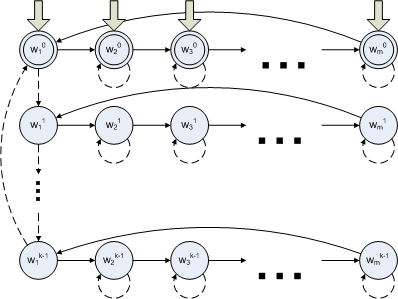
\includegraphics[width = 8cm, bb= 0 0 398 299]{autom_km.png}
  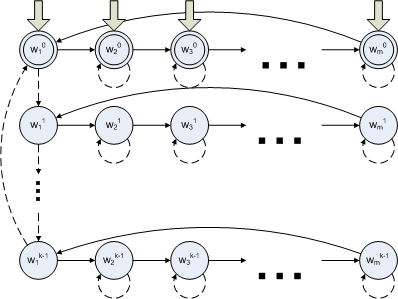
\includegraphics[width = 8cm]{autom_km.png}
  \caption{Ultrametric automaton recognizing $L_{k,m}$ with $k \cdot m$ states.
  Double circled states are final.
  Big arrows show starting states.
  Solid lines are $a$-transitions, dashed lines are $b$-transitions.
  All transitions have amplitude 1. }
  \label{autom1}
\end{figure}

We can do even better if we use the ultrametric properties of the automaton.

\begin{theorem}
For every prime $p > m$ there is an integral $p$-ultrametric finite automaton recognizing $L_{p,m}$ with $m+1$ states.
\end{theorem}
\begin{proof}
The automaton has states $w_i$ where $i \in \{1, \ldots, m\}$ and a starting state "$1$" which has always amplitude $1$.
The automaton is constructed in such way that after reading word $x$ the state $w_i$ contains an amplitude divisible by $p$ iff $f_x(0^m)_i = 0$.
Therefore, if $x \in L$ the sum of norms of the amplitudes of the final states is less than $m \cdot p^{-1}$. Otherwise that sum is greater than $1$.

See figure \ref{autom2}.
\qed
\end{proof}


\begin{figure}[H]
  \centering
  % 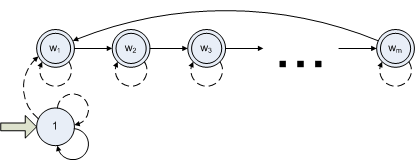
\includegraphics[width = 8.4cm, bb= 0 0 415 160]{autom_m1.png}
  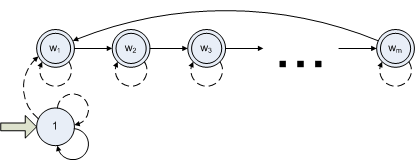
\includegraphics[width = 8.4cm]{autom_m1.png}
  \caption{$p$-ultrametric automaton recognizing $L_{p,m}$ with $m$ states.
  Double circled states are final.
  Big arrow shows the starting state.
  Solid lines are $a$-transitions, dashed lines are $b$-transitions.
  All transitions have amplitude 1. }
  \label{autom2}
\end{figure}


\begin{theorem}
(1) If a language $M$ is recognized by a regulated, integral $p$-ultrametric finite automaton then $M$ is regular.\\
(2) For arbitrary prime number $p$ there is a constant $c_p$ such that if a language $M$ is recognized by a regulated $p$-ultrametric finite automaton with $k$ states then there is a deterministic finite automaton with $(c_p)^{k\cdot \log k}$ states recognizing the language $M$.
\end{theorem}
\begin{proof}
If the automaton is regulated then, for arbitrary input word $x$, the norm  $|\gamma |_p$ is in the interval $0 < \rho -c < |\gamma |_p < \rho +c$. This means that there is only a finite number of possible values of the amplitudes of the final states. Namely, the amplitude of each final state can take no more than $p^{const}$ values, and there is a constant $d$ such that only the last $d$ digits of the amplitudes (being $p$-adic numbers) of these states can influence  the norm.

Since amplitudes after each step of the computation are calculated as elements of a matrix product, and the elements of the matrices are $p$-adic numbers, only the last $d$ digits of the amplitudes of all the states can influence the result. Hence all the information about any initial fragment of the input word is encoded in the last $d$ digits of the amplitudes of all the states. No more than $(c_p)^{k\log k}$ possibilities can be distinguished.
\end{proof}


\begin{thebibliography}{99}

\bibitem{DD09}
Branko Dragovich and Alexandra Dragovich.
A $p$-Adic Model
of DNA Sequence and Genetic Code.
{\em $p$-Adic Numbers, Ultrametric Analysis, and Applications,}
vol. 1, No 1, 34--41, 2009

\bibitem{F12}
R\= usi\c n\v s Freivalds.
{\em Ultrametric automata and Turing machines.} Proceedings of The Alan Turing Centenary Conference, 2012.

\bibitem{H01}
Mika Hirvensalo.
{\em Quantum Computing.} Springer-Verlag, Berlin-Heidelberg,  2001.

\bibitem{Kh97}
Andrei Yu. Khrennikov.
{\em Non�Archimedean Analysis: Quantum Paradoxes, Dynamical Systems and
Biological Models,} Kluwer Academic Publishers, 1997.
	
\bibitem{K06}
Sergey V. Kozyrev. 
Ultrametric Analysis and Interbasin Kinetics.
{\em $p$-Adic Mathematical Physics,} Proc. of the 2nd International Conference on $p$-Adic 
Mathematical Physics, American Institute Conference Proceedings,
vol. 826, pp. 121--128, 2006.

\bibitem{M00}
David A. Madore.
{\em A first introduction to $p$-adic numbers}. Available online: \url{http://www.madore.org/\textasciitilde david/math/padics.pdf}.

\bibitem{T69}
Paavo Turakainen.
Generalized Automata and Stochastic Languages.
{\em Proceedings of the American Mathematical Society,} vol. 21, No. 2, pp. 303--309, 1969.

\bibitem{VVZ95}
V. S. Vladimirov, I. V. Volovich and E. I. Zelenov.
{\em $p$-Adic Analysis and Mathematical Physics} 
World Scientific, Singapore, 1995. 

\end{thebibliography}


\end{document}
